\begin{slide}{Current Work}
	Original motivation from Summer 2020 IPRO with Prof. Robert Ellis and Mr. David Eads (NPR). \\
	Expanded over Summer 2021 with Prof. Chun Liu and Prof. Yiwei Wang. \\
	
	\vspace{.5cm}
	
	{\large Start by defining the zero-dimension (ODE) model:}
	\begin{enumerate}
		\item Start with a population of \emph{susceptibles} ($S$)
		\item Some of the population may become \emph{infected} ($I$) upon emergence of the virus
		\item Infected individuals interact with susceptibles at rate $\beta$ to draw new members into $I$
		\item A fraction of $I$ recover or die at a rate $\gamma$ moving to the \emph{removed} ($R$) population
	\end{enumerate}
	\begin{figure}
		\centering
		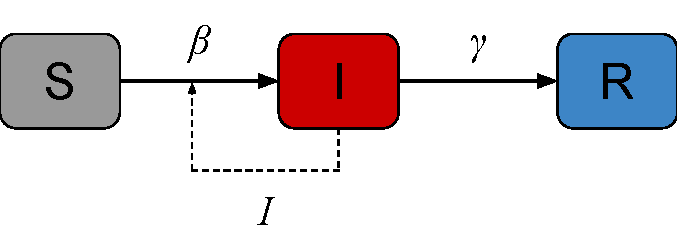
\includegraphics[height=3cm]{images/sir_schematic}
	\end{figure}
	This represents processes that occur in a ``well mixed'' situation.
\end{slide}